<<<<<<< 748b67fd60b26d45750e10209255345ebe612814
\section{Durchführung}
\label{sec:Durchführung}
||||||| merged common ancestors
\section{Durchführung}
\label{sec:Durchführung}
=======
\section{Durchführung}
\begin{figure}[H]
  \centering
  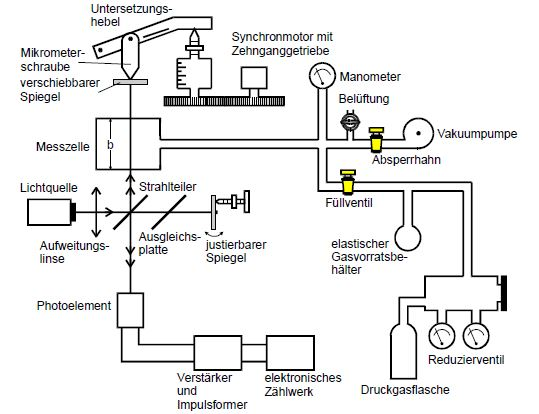
\includegraphics[height=7cm]{aufbau.JPG}
  \caption{Aufbau der verwendeten Mesaperatur}
  \label{fig:aufbau}
  \cite{skript}.
\end{figure}
Bevor die Messungen durchgeführt werden können, muss die Aperatur justiert werden.
Dazu werden die Spiegel mit Hilfe der Rändelschrauben so verstellt, dass die beiden hellsten
Strahlen die aus dem Interferometer kommen sich überlagern. Am besten werden die Strahlen mit
einem Stück Papier im Strahlengang sichtbar gemacht. Der Detektor wird nun auf die
Position eingestellt, in der sich die Strahlen überlagern.

Um nun die Wellenlänge des verwendeten Lasers zu messen wir ein Spiegel mit Hilfe eines Motors
und einer Mikrometrschraube langsam verschoben. Wichtig ist, dass sich der Spiegel nicht zu schnell
bewegt, damit das Photoelement alle Maxima regestrieren kann. Der Spiegel wird in jeder
Messung um $\SI{3}{\mm}$ verschoben, die Messung wird fünfmal wiederholt. Nach jeder Messung
wird die Anzahl der regestrieren Maxima notiert.\\
Um den Brechungsindex von Luft zu bestimmen bleiben beide Spiegel in Ruhe.
Die Kammer wird mit einer Handpumpe auf einen Druck $p$ evakuiert, dieser Druck wird notiert.
Nun wird die Luft wieder eingelassen und das Photoelement regestriert die Maxima, diese werden
ebenfalls notiert. Diese Messung wird zehnmal wiederholt.



\label{sec:Durchführung}
>>>>>>> michelson
